\documentclass{article}

\usepackage[english]{babel}
\usepackage[letterpaper,top=2.5cm,bottom=2.5cm,left=2.5cm,right=2.5cm,marginparwidth=1.75cm]{geometry}
\usepackage{amsmath, fancyhdr, graphicx, pgfplots}
\usepackage[colorlinks=true, allcolors=black]{hyperref}

\pagestyle{fancy}
\fancyhf{}
\rhead{11/1/22\\Jacob Sigman}
\lhead{CE-344\\Environmental Systems Engineering}
\cfoot{\thepage}
\renewcommand{\headrulewidth}{1.5pt}
\setlength{\headheight}{22.6pt}

\begin{document}
    \thispagestyle{plain}
    {\LARGE{\noindent \bf CE-344 Homework\\\\}}
    {\Large{Jacob Sigman\\\\}}
    \tableofcontents
    \newpage
    % \part*{Week 2}
\section*{Chapter 2}
\underline{1-6, 9-13, 17, 26}
\subsection*{Problem 1}
Using atomic weights given in Table 1, calculate the molecular and equivalent weights of \\(a) alum
(\(\textnormal{Al}_2(\textnormal{SO}_4)_3\cdot 14.3\textnormal{H}_2\textnormal{O}\)), (b) lime, (c) ferrous sulfate (FeS\(\textnormal{O}_4\)\(\cdot\)7\(\textnormal{H}_2\)O), (d) fluorosilicic acid, and (e) soda ash.\\
\rule{5cm}{1pt}
\begin{description}
    \item [(a)]\[\textnormal{Atomic Weight} = 2\times 27+3\times 96+14.3\times(2+16)=\boxed{600\textnormal{ amu}}\]
    \[\textnormal{Total Valence: } 3\times 2 = 6\]
    \[\textnormal{Equivalent Weight} = \frac{600}{6}=\boxed{100\textnormal{ amu}}\]
    \item [(b)]
    \[\textnormal{Atomic Weight} =\boxed{56.1\textnormal{ amu}}\]
    \[\textnormal{Equivalent Weight} =\boxed{28\textnormal{ amu}}\]
    \item [(c)]
    \[\textnormal{Atomic Weight} =\boxed{278\textnormal{ amu}}\]
    \[\textnormal{Equivalent Weight} =\boxed{139\textnormal{ amu}}\]
    \item [(d)]
    \[\textnormal{Atomic Weight} =\boxed{144\textnormal{ amu}}\]
    \[\textnormal{Equivalent Weight} =\boxed{\textnormal{N/A}}\]
    \item [(e)]
    \[\textnormal{Atomic Weight} =\boxed{106\textnormal{ amu}}\]
    \[\textnormal{Equivalent Weight} =\boxed{53\textnormal{ amu}}\]
\end{description}
\subsection*{Problem 2}
What ions are formed when the following compounds dissolve in water: (a) sodium nitrate, (b) sulfuric acid, (c) calcium hypochlorite, and (d) sodium carbonate.\\
\rule{5cm}{1pt}
\begin{description}
    \item [(a)]
    \[\boxed{\textnormal{Na}^+\textnormal{ and NO}_3^-}\]
    \item [(b)]
    \[\boxed{\textnormal{2H}^+\textnormal{ and HSO}_4^-}\]
    \item [(c)]
    \[\boxed{\textnormal{Ca}^{++}\textnormal{ and 2OCl}^-}\]
    \item [(d)]
    \[\boxed{\textnormal{2Na}^+\textnormal{ and CO}_3^{=}}\]
\end{description}
\subsection*{Problem 3}
All of the fluoridation chemicals listed in Table 2-3 yield \(\textnormal{F}^-\) ions in solution. If 1.0 mg of fluorosilicic acid is added to water, what is the increase in concentration?\\
\rule{5cm}{1pt}
\[\textnormal{Ratio of Fluorine in Fluorosilicic Acid}=\frac{6\times 19\textnormal{ amu}}{144\textnormal{ amu}}=0.79\]
\[\textnormal{Concentration}=1\textnormal{ mg}\times 0.79=\boxed{0.79 \textnormal{ mg/L}}\]
\subsection*{Problem 4}
If a water contains 29 mg/L of \(\textnormal{Ca}^{++}\) and 16.4 mg/L of \(\textnormal{Mg}^{++}\), what is the hardness expressed in milligrams per liter as CaC\(\textnormal{O}_3\)?\\
\rule{5cm}{1pt}
\[\textnormal{Hardness of }\textnormal{Ca}^{++}\textnormal{ and Mg}^{++}=29\textnormal{ mg/L}\,\frac{\textnormal{EW CaCO}_3\textnormal{ amu}}{\textnormal{EW Ca amu}}+16.4\textnormal{ mg/L}\,\frac{\textnormal{EW CaCO}_3\textnormal{ amu}}{\textnormal{EW Mg amu}}\]
\[\textnormal{Hardness of }\textnormal{Ca}^{++}\textnormal{ and Mg}^{++}=29\textnormal{ mg/L}\,\frac{50\textnormal{ amu}}{20\textnormal{ amu}}+16.4\textnormal{ mg/L}\,\frac{50\textnormal{ amu}}{12.2\textnormal{ amu}}=\boxed{140\textnormal{ mg/L}}\]
\subsection*{Problem 5}
If a water contains 175 mg/L of calcium hardness and 40 mg/L of magnesium hardness, what are the concentrations of \(\textnormal{Ca}^{++}\) and \(\textnormal{Mg}^{++}\) ions?\\
\rule{5cm}{1pt}
\[\textnormal{Ca}^{++}=\textnormal{EW Ca amu}\,\frac{\textnormal{Ca Hardness mg/L}}{\textnormal{EW CaCO}_3\textnormal{ amu}}=20\textnormal{ amu}\,\frac{175\textnormal{ mg/L}}{50\textnormal{ amu}}=\boxed{70 \textnormal{ mg/L}}\]
\[\textnormal{Mg}^{++}=\textnormal{EW Mg amu}\,\frac{\textnormal{Mg Hardness mg/L}}{\textnormal{EW CaCO}_3\textnormal{ amu}}=12.2\textnormal{ amu}\,\frac{40\textnormal{ mg/L}}{50\textnormal{ amu}}=\boxed{9.8 \textnormal{ mg/L}}\]
\subsection*{Problem 6}
The alkalinity of a water consists of 12 mg/L of C\(\textnormal{O}_3^-\) and 100 mg/L of HC\(\textnormal{O}_3^-\). Calculate the alkalinity in milligrams per liter as CaC\(\textnormal{O}_3\).\\
\rule{5cm}{1pt}
\[\textnormal{Alkalinity }=\textnormal{mg/L CO}_3\,\frac{\textnormal{EW CaCO}_3\textnormal{ amu}}{\textnormal{EW CO}_3\textnormal{ amu}}+\textnormal{mg/L HCO}_3\,\frac{\textnormal{EW CaCO}_3\textnormal{ amu}}{\textnormal{EW HCO}_3\textnormal{ amu}}\]
\[\textnormal{Alkalinity }=12\textnormal{ mg/L}\,\frac{50\textnormal{ amu}}{30\textnormal{ amu}}+100\textnormal{ mg/L}\,\frac{50\textnormal{ amu}}{61\textnormal{ amu}}=\boxed{102\textnormal{ mg/L}}\]
\newpage
\subsection*{Problem 9}
Draw a milliequivalents-per-liter bar graph for the following water analysis:\\\\
\begin{tabular}{l l}
    C\(\textnormal{a}^{++}\) = 60 mg/L & HC\(\textnormal{O}_{3}^-\) = 115 mg/L as CaC\(\textnormal{O}_3\) \\
    M\(\textnormal{g}^{++}\) = 10 mg/L & S\(\textnormal{O}_{4}^{=}\) = 96 mg/L \\
    N\(\textnormal{a}^{+}\) = 7 mg/L  &  C\(\textnormal{l}^{-}\) = 11 mg/L \\
    \(\textnormal{K}^{+}\) = 20 mg/L &
\end{tabular}
\\\\
\rule{5cm}{1pt}
\begin{center}
\begin{tabular}{l c c c}
    Molecule & mg/L & EW & meq/L\\
    \hline
    Ca & 60 & 20 & 3\\
    Mg & 10 & 12.2 & 0.8\\
    Na & 7 & 23 & 0.3\\
    K & 20 & 39.1 & 0.5\\
    HC\(\textnormal{O}_3\) & 115 & 50 & 2.3\\
    S\(\textnormal{O}_4\) & 96 & 48 & 2\\
    Cl & 11 & 35.5 & 0.3
\end{tabular}\\
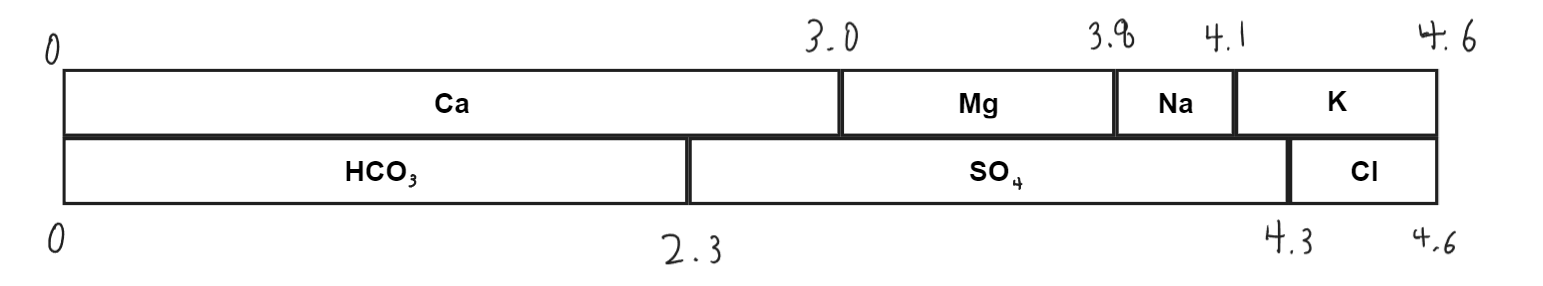
\includegraphics[scale=0.3]{diagram1.png}
\end{center}

\subsection*{Problem 10}
A brackish groundwater in an arid region has the following chemical characteristics:\\\\
\begin{tabular}{l l}
    C\(\textnormal{a}^{++}\) = 108 mg/L & HC\(\textnormal{O}_{3}^-\) = 146 mg/L \\
    M\(\textnormal{g}^{++}\) = 44 mg/L & S\(\textnormal{O}_{4}^{-2}\) = 110 mg/L \\
    N\(\textnormal{a}^{+}\) = 138 mg/L  &  C\(\textnormal{l}^{-}\) = 366 mg/L\\
\end{tabular}
\\\\
Draw the milliequivalents-per-liter bar graph. Calculate the carbonate hardness (associated with the bicarbonate ion), noncarbonated hardness, total hardness, sodium ion concentration, and alkalinity.
\\
\rule{5cm}{1pt}
\begin{center}
\begin{tabular}{l c c c}
    Molecule & mg/L & EW & meq/L\\
    \hline
    Ca & 108 & 20 & 5.4\\
    Mg & 44 & 12.2 & 3.6\\
    Na & 138 & 23 & 6\\
    HC\(\textnormal{O}_3\) & 146 & 61 & 2.4\\
    S\(\textnormal{O}_4\) & 110 & 48 & 2.3\\
    Cl & 366 & 35.5 & 10.3
\end{tabular}\\
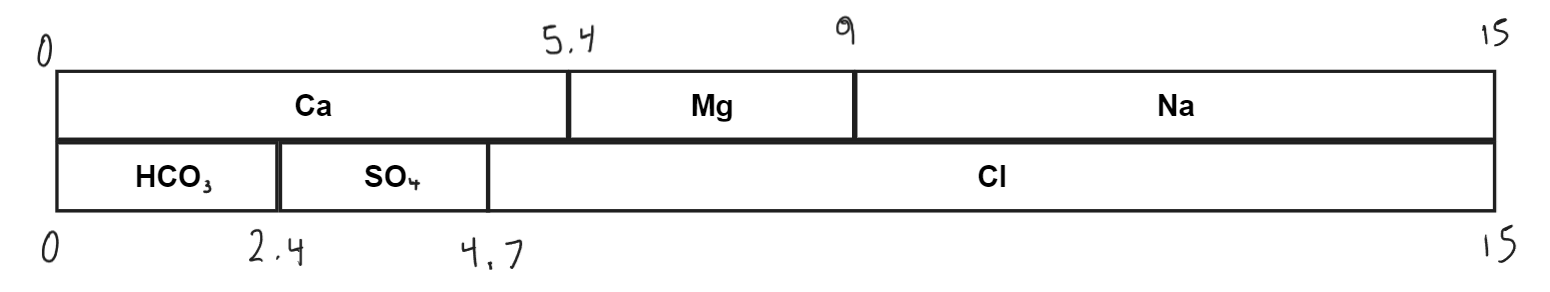
\includegraphics[scale=0.33]{diagram2.png}
\end{center}
\[\textnormal{Carbonate Hardness }=2.4\textnormal{ meq/L}\times 50\textnormal{ amu}=\boxed{120 \textnormal{ mg/L}}\]
\[\textnormal{Noncarbonate Hardness }=(5.4\textnormal{ meq/L}-2.4\textnormal{ meq/L})\times 50\textnormal{ amu}=\boxed{150 \textnormal{ mg/L}}\]
\[\textnormal{Total Hardness }=9\textnormal{ meq/L}\times 50\textnormal{ amu}=\boxed{450 \textnormal{ mg/L}}\]
\[\textnormal{Alkalinity }=2.4\textnormal{ meq/L}\times 50\textnormal{ amu}=\boxed{120 \textnormal{ mg/L}}\]
\newpage
\subsection*{Problem 11}
Draw a milliequivalents-per-liter graph and list the hypothetical combinations of chemicals in solution for the following:\\\\
\begin{tabular}{l c l}
    Calcium hardness & = & 150 mg/L \\
    Magnesium hardness & = & 65 mg/L \\
    Sodium ion & = & 8 mg/L \\
    Potassium ion & = & 4 mg/L \\
    Alkalinity & = & 190 mg/L \\
    Sulfate ion & = & 29 mg/L \\
    Chloride ion & = & 10 mg/L \\
    pH & = &  7.7
\end{tabular}
\\\\\rule{5cm}{1pt}
\begin{center}
\begin{tabular}{l c c c}
    Molecule & mg/L & EW & meq/L\\
    \hline
    Ca & 150 & 50 & 3\\
    Mg & 65 & 50 & 1.3\\
    Na & 8 & 23 & 0.3\\
    K & 4 & 39.1 & 0.1\\
    HC\(\textnormal{O}_3\) & 190 & 50 & 3.8\\
    S\(\textnormal{O}_4\) & 29 & 48 & 0.6\\
    Cl & 10 & 35.5 & 0.3
\end{tabular}\\
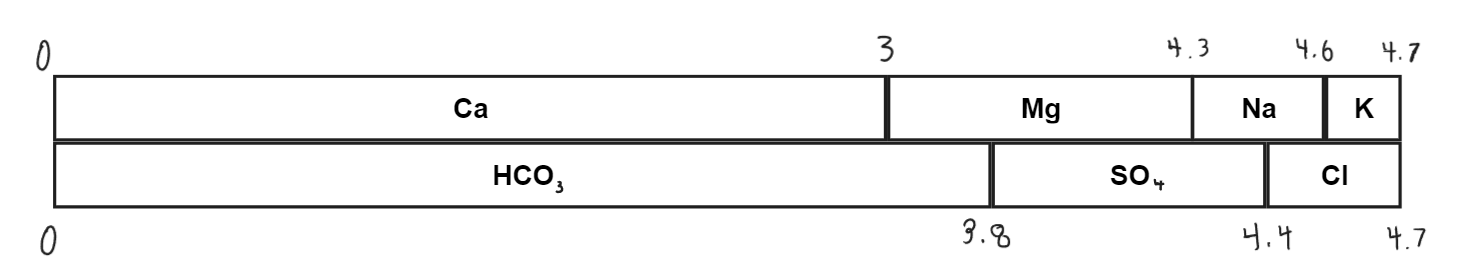
\includegraphics[scale=0.33]{diagram3.png}
\end{center}
\[\textnormal{Combinations (in meq/L): } \boxed{3 \textnormal{ Ca(HCO}_3)_2,\,0.8 \textnormal{ Mg(HCO}_3)_2,\,0.5\textnormal{ MgSO}_4,\,0.1\textnormal{ Na}_2\textnormal{SO}_4,\,0.2\textnormal{ NaCl},\,0.1\textnormal{ KCl}}\]
\subsection*{Problem 12}
A sulfuric acid solution is added to scale-forming water to convert calcium carbonate to calcium bicarbonate. Write the chemical equation for this reaction, and calculate the amount of sulfuric acid in milligrams per liter to neutralize 20 mg/L of calcium carbonate.\\
\rule{5cm}{1pt}
\[\textnormal{Balanced Reaction: }\boxed{\textnormal{H}_2\textnormal{SO}_4+2\textnormal{CaCO}_3\,\rightarrow\,\textnormal{Ca(HCO}_3)_2+\textnormal{CaSO}_4}\]
\[\textnormal{Molecular Weight CaCO}_3=100\times 2=200\textnormal{ amu}\]
\[\textnormal{Molecular Weight H}_2\textnormal{SO}_4=98.1\times 1=98.1\textnormal{ amu}\]
\[\frac{\textnormal{mg/L CaCO}_3}{\textnormal{Molecular Weight CaCO}_3}=\frac{\textnormal{mg/L H}_2\textnormal{SO}_4}{\textnormal{Molecular Weight H}_2\textnormal{SO}_4}\]
\[\frac{20\textnormal{ mg/L}}{\textnormal{200 amu}}=\frac{x \textnormal{ mg/L H}_2\textnormal{SO}_4}{98.1\textnormal{ amu}}\]
\[x=\boxed{9.81\textnormal{ mg/L}}\]
\subsection*{Problem 13}
Calculate the pH of a solution containing 10 mg/L of sulfuric acid.\\
\rule{5cm}{1pt}
\[\textnormal{Molecular Weight H}_2\textnormal{SO}_4=98.1\textnormal{ amu}\]
\[\textnormal{H}^+=\frac{1 \textnormal{ g}}{10 \textnormal{ mg}}\div 98.1\textnormal{ amu}=1.01\times 10^{-4}\textnormal{ g/L}\]
\[\textnormal{pH}=-\log(\textnormal{H}^+)=-\log(1.01\times 10^{-4})=\boxed{4}\]
\subsection*{Problem 17}
In softening of water, lime slurry Ca(OH\()_2\) is added to precipitate the calcium ion, associated with the bicarbonate radical, as CaC\(\textnormal{O}_3\). Write a balanced equation for this reaction. Calculate the amount of lime as calcium oxide necessary to react with 100 mg/L of calcium hardness.\\
\rule{5cm}{1pt}
\[\textnormal{Balanced Reaction: }\boxed{\textnormal{Ca(OH)}_2+\textnormal{Ca(HCO}_3\textnormal{)}_2\,\rightarrow\,2\textnormal{CaCO}_3+2\textnormal{H}_2\textnormal{O}}\]
\[\frac{\textnormal{EW CaO amu}}{\textnormal{EW CaCO}_3\textnormal{ amu}}=\frac{x\textnormal{ mg/L CaO}}{\textnormal{mg/L CaCO}_3}\]
\[\frac{28\textnormal{ amu}}{50\textnormal{ amu}}=\frac{x\textnormal{ mg/L CaO}}{100\textnormal{ mg/L}}\]
\[x=\boxed{56\textnormal{ mg/L}}\]
\subsection*{Problem 26}
In Eq. 29, why is the value of the constant 50,000 to calculate alkalinity as CaC\(\textnormal{O}_3\)?\\
\rule{5cm}{1pt}
\[\textnormal{Alkalinity }=\frac{\textnormal{mL Titrant}\times\textnormal{Normality of Acid}\times x}{\textnormal{mL Sample}}\]
Where, according to the textbook, the volume of the titrant is 1 mL, the volume of the sample is 100 mL, the alkalinity is 10 mg/L, and the normality of the acid is 0.02 N.
\[\textnormal{10 mg/L}=\frac{1\textnormal{ mL}\times 0.02\textnormal{ N}\times x}{\textnormal{100 mL}}\]
\[x=\frac{\textnormal{10 mg/L}\times\textnormal{100 mL}}{1\textnormal{ mL}\times 0.02\textnormal{ N}}=\boxed{50000}\]
    % \part*{Week 3}
\section*{Chapter 3}
\underline{15-17, 20-23, 26}
\subsection*{Problem 15}
Compare the latency, persistence, and infective dose of \emph{Ascaris} and \emph{Salmonella}.
\subsection*{Problem 16}
Historically in the United States, the prevalent infectious diseases were typhoid, cholera, and dysentery. How have these diseases been virtually eliminated? Currently, the prevalent infectious diseases are giardiasis and cryptosporidiosis, causing diarrhea that can be life-threatening for persons with immunodeficiency syndrome. What actions are being taken to reduce the probability of waterborne transmission of these diseases? (Refer to Section 5.)
\subsection*{Problem 17}
Discuss the significance of human carriers in transmission of enteric diseases. What major waterborne diseases in the United States are spread by carriers? How is the spread of two of these diseases amplified by animals?
\subsection*{Problem 20}
In one statement, what is the general process in testing for \emph{Giardia} cysts and \emph{Cryptosporidium} oocysts? In method 1622, the water sample is only 10 L for testing natural stream water for \emph{Cryptosporidium} oocysts. Using this method to test stream samples at a variety of locations, why was the accuracy for detection and enumeration of oocysts low?
\subsection*{Problem 21}
Why must laboratories conducting tests for \emph{Cryptosporidium} oocysts be audited and approved for quality assurance?
\subsection*{Problem 22}
Why are coliform bacteria used as indicators of quality of drinking water? Under what circumstances is the reliability of coliform bacteria to indicate the presence of pathogens questioned?
\subsection*{Problem 23}
Coliform bacteria in surface waters can originate from feces of humans, wastes of farm animals, or soil erosion. Can the coliforms from these three different sources be distinguished from one another?
\subsection*{Problem 26}
Why is lactose (milk sugar), an ingredient in all culture media, used to test for the coliform group?
    % \part*{Week 4}
\addcontentsline{toc}{part}{Week 4}
\section*{Chapter 5}
\underline{9-14}
\addcontentsline{toc}{section}{Chapter 5: 9-14}
\subsection*{Problem 9}
How is monitoring conducted for lead and copper in drinking water? What are the action levels, and what are the treatment techniques if these action levels are exceeded?
\\\rule{5cm}{1pt}
\\\\Monitoring is conducted for lead and copper in first-flush tap samples. The action level for lead is 0.015 mg/L and the action level for copper is 1.3 mg/L. The treatment technique is to perform corrosion studies. Additionally, a public education program on the many health risks and actions that can be taken to reduce water pollution is required.
\subsection*{Problem 10}
What is the optimum concentration of fluoride in drinking water in a location where the average maximum daily air temperature is 60°F? What is the health benefit of drinking water containing the optimum concentration of fluoride?
\\\rule{5cm}{1pt}
\\\\The optimum concentration of fluoride in drinking water in a location where the maximum daily air temperature is 60°F is 1 mg/L. The optimum concentration of fluoride in drinking water prevents teeth from decay. 
\subsection*{Problem 11}
What is the health risk of nitrate in drinking water?
\\\rule{5cm}{1pt}
\\\\The health risk fo nitrate in drinking water is Methemoglobinemia in infants 3 to 6 months of age.
\subsection*{Problem 12}
What are the most frequently detected VOCs in contaminated groundwater? What pesticide SOCs have been detected in groundwater?
\\\rule{5cm}{1pt}
\\\\The most frequently detected VOCs in contaminated groundwater are \textit{trichloroethylene}, \textit{tetrachloroethylene}, \textit{carbon tetrachloride}, \textit{1,1, 1-trichloroethane}, \textit{1, 2-dichloroethane}, and \textit{vinyl chloride}. THe pesticide SOCs that have been detected in groundwater are \textit{alachlor}, \textit{aldicarb}, \textit{atrazine}, \textit{carbofuran}, \textit{ethylene dibromide}, and \textit{dibromochloropropane}.
\newpage
\subsection*{Problem 13}
Write the chemical formulas for the five trihalomethane compounds that have been found in drinking water. What is the source of the THMs?
\\\rule{5cm}{1pt}
\begin{enumerate}
    \item \(\text{CHCl}_3\)
    \item \(\text{CHBrCl}_2\)
    \item \(\text{CHBr}_2\text{Cl}\)
    \item \(\text{CHBr}_3\)
    \item \(\text{CHCl}_2\text{I}\)
\end{enumerate}
The source of THMs is the treatment of surface waters, particularly with chlorination. 
\subsection*{Problem 14}
Why are iron and manganese included in secondary standards for aesthetics?
\\\rule{5cm}{1pt}
\\\\Iron and manganese are included in secondary standards for aesthetics due to the brownish-colored staining of laundry and porcelain.


    % \part*{Week 5}
\addcontentsline{toc}{part}{Week 5}
\section*{Chapter 6}
\underline{2-5, 19}
\addcontentsline{toc}{section}{Chapter 6: 2-5, 19}
\subsection*{Problem 2}
Based on demand of 100 gpcd, estimate the maximum daily demand and the mean maximum hourly rate.
\\\rule{5cm}{1pt}
\[\text{Maximum daily demand}=1.8\times100=\boxed{180\text{ gpcd}}\]
\[\text{Mean maximum hourly rate}=3\times100=\boxed{300\text{ gpcd}}\]
\subsection*{Problem 3}
What is the range of water pressure recommended in a distribution system? What are the minimum and maximum pressures for residential service connections?
\\\rule{5cm}{1pt}
\\\\The range of recommended water pressure in a distribution system is 65 to 75 psi. The minimum and maximum pressures for residential service connections are 40 and 100 psi respectively.
\subsection*{Problem 4}
Define needed fire flow. Based on Eq. 4, list the factors taken into consideration in determining NFF.
\\\rule{5cm}{1pt}
\\\\Needed fire flow is the rate of water flow required for firefighters to ensure that major fires remain within a block with minimal loss. The factors taken into consideration in determining needed fire flow are: construction type, area of the floor of the building, involvement with other buildings, and occupancy.
\subsection*{Problem 5}
A wood-frame building on the first floor is a restaurant with floor dimensions of 30 ft by 75 ft (2250 sq ft). On one end of the second floor is a cabinet-making shop 30 ft by 30 ft (900 sq ft). The building has two sides with exposures to adjacent buildings. Opposite the long side of the restaurant at a distance of 11 ft is building A with two-story masonry walls and semiprotected openings. The length–height measurement is \(120\times2=240\text{ ft}\times\text{stories}\). The second exposure is building B with a width of 28 ft at a distance of 12 ft from the end of the restaurant. The building is constructed of frame walls with two stories for a length–height measurement of \(28\times2=56\text{ ft}\times\text{stories}\). Calculate the NFF for the restaurant-cabinet shop.
\\\rule{5cm}{1pt}
\[NFF=C_i\times O_i\times[1.0+(X_i+P_i)]\]
\[C_i=18F\sqrt{A_i}\text{ where }F=1.5\text{ and } A_i=2250\text{ ft}^2+0.5*900\text{ ft}^2=2700\text{ ft}^2\]
\[C_i=1400,\,\, O_i=1.15,\,\, X_i=0.18,\,\, P_i=0\]
\[NFF=\boxed{1900 \text{ gpm}}\]
\newpage
\subsection*{Problem 19}
A new vertical-turbine well pump is being installed to discharge groundwater directly into the pipe network of a small community. Operating head-discharge data based on specifications from the pump manufacturer are 210 gpm discharge at a pump head of 170 ft measured from ground level, 300 gpm at 165 ft, 410 gpm at 150 ft, and 470 gpm at 130 ft. The water pressure at ground level into the pipe network varies from 71 psi to 48 psi, with an average pressure of 64 psi. Plot the head-discharge curve and locate the pressure range and average value. What is the pump discharge against the average pressure of 64 psi?
\\\rule{5cm}{1pt}
\begin{center}
\begin{tikzpicture}[baseline=(current bounding box.center)]
    \begin{axis}[
        title={\textbf{Head-Discharge Curve}},
        xlabel={gpm},
        ylabel={ft},
        xmin=200, xmax=500,
        ymin=130, ymax=170,
        xtick={200,300,400,500},
        ytick={130,140,150,160,170},
        ymajorgrids=true,
        grid style=dashed,
    ]
    
    \addplot[mark=square, black] table [x=x, y=y] {curve.csv};
    % \addplot[no markers, red, domain=0:1.27] {8.8656*x*x*x-17.653*x*x+3.6097*x+7.385};
    \end{axis}
\end{tikzpicture}
\end{center}
\[\text{Average: }=\frac{170+165+150+130}{4}=\boxed{150\text{ ft}}\]
\[\text{Pump Discharge: }=\boxed{400\text{ gpm}}\]
\newpage
\section*{Chapter 7}
\underline{3-5, 13-14, 26-31}
\addcontentsline{toc}{section}{Chapter 7: 3-5, 13-14, 26-31}
\subsection*{Problem 3}
A flocculator designed to treat 10 mgd is 48 ft long, 52 ft wide, and 12 ft deep. Compute the detention time and horizontal flow-through velocity. Do these values satisfy the \textit{Standards for Water Works}?
\\\rule{5cm}{1pt}
\[t=\frac{V}{Q}=\frac{48\text{ ft}\times52\text{ ft}\times12\text{ ft}\times7.48\,\frac{\text{gal}}{\text{ft}^3}\times1440\,\frac{\text{minutes}}{\text{day}}}{10000000\,\frac{\text{gal}}{\text{day}}}=\boxed{32\text{ minutes}}\]
\[v=\frac{L}{t}=\frac{48\text{ ft}}{32\text{ minutes}}=\boxed{1.5\text{ ft/min}}\]
\begin{center}
Both of these values satisfy the \textit{Standards for Water Works}.
\end{center}
\subsection*{Problem 4}
Locate the rapid-mixing chambers, flocculation basins, and settling tanks in Figure 4a. If this plant as pictured had been designed for 30 mgd (15 mgd for each side) based on the \textit{Standards for Water Works}, what would be the volumes of the rapid mixers, flocculation basins, and sedimentation tanks?
\\\rule{5cm}{1pt}
\[\text{Volume of rapid mixer}=30\text{ seconds}\times30\text{ mgd}\times1000000 \text{ gal}\times\,\frac{1 \text{ day}}{86400 \text{ seconds}}=\boxed{10416 \text{ gal}}\]
\[\text{Volume of flocculation basin}=30\text{ minutes}\times30\text{ mgd}\times1000000 \text{ gal}\times\,\frac{1 \text{ day}}{1440 \text{ minutes}}=\boxed{625000 \text{ gal}}\]
\[\text{Volume of sedimentation tank}=4\times30\text{ mgd}\times\frac{1 \text{ day}}{24\text{ hours}}=\boxed{5000000 \text{ gal}}\]
\subsection*{Problem 5}
Calculate the detention time and overflow rate for a sedimentation basin with a volume of 1.0 mil gal and surface area of 12,500 sq ft treating 8.0 mgd. 
\\\rule{5cm}{1pt}
\[t=\frac{V}{Q}=\frac{1000000\text{ gal}\times24}{8\text{ mgd}}=\boxed{3\text{ hours}}\]
\[V_0=\frac{Q}{A}=\frac{8\text{ mgd}}{12500\text{ ft}^2}=\boxed{640\text{ gpd/ft}^2}\]
\newpage
\subsection*{Problem 13}
Flocculator-clarifiers similar to the one illustrated in Figure 10 are proposed for precipitation in lime– soda ash softening of a groundwater. The inside diameter of the tank is 40 ft and sidewater depth is 10 ft. The cone-shaped skirt is 12 ft in diameter at the water surface and 24 ft in diameter at the bottom, which is at a depth of 8.0 ft below the water surface. The design flow for each flocculator-clarifier is 750,000 gpd. Does this proposed design meet the \textit{Standards for Water Works} for detention times based on total volume, mixing and flocculation time, and upflow rate based on the open-water surface area? (The cone-shaped shirt can be considered to be the geometric form of a conical basin illustrated in the appendix.)
\\\rule{5cm}{1pt}
\[V_\text{tank}=\pi\times20^2\times10=12600\text{ ft}^3=94254\text{ gal}\]
\[V_\text{skirt}=\frac{1}{3}\times\pi\times8\times(6^2+6\times12+12^2)=2111\text{ ft}^3=15791\text{ gal}\]
\[t_\text{tank}=\frac{94000\text{ gal}}{750000\text{ gpd}\times\frac{1 \text{ day}}{1440 \text{ hours}}}=3\text{ hours}\]
\[t_\text{skirt}=\frac{15800}{750000\text{ gpd}\times\frac{1 \text{ day}}{86400 \text{ minutes}}}=30 \text{ minutes}\]
\[V_0=\frac{750000\text{ gpd}\times\frac{1 \text{ day}}{86400 \text{ minutes}}}{\pi(20^2-6^2)}=0.46\text{ gpm/ft}^2\]
\begin{center}
    All of these values satisfy the \textit{Standards for Water Works}.
\end{center}
\subsection*{Problem 14}
The settling velocity of calcium carbonate floc formed during flocculation in a flocculator-clarifier (Figure 10) is 2.1 mm/s. If the detention time in the settling zone is 1.0 hr and upflow rate is 1.75 gpm/sq ft, what is the minimum depth of water required to ensure removal of the floc by gravity settling?
\\\rule{5cm}{1pt}
\[\left[\left(2.1\times\frac{1 \text{ mm}}{304.8 \text{ ft}}\right)-\left(1.75\times\frac{1 \text{ gal}}{7.48 \text{ ft}^3}\times\frac{1 \text{ minute}}{60\text{ seconds}}\right)\right]\times3600\text{ seconds}=\boxed{10\text{ ft}}\]
\subsection*{Problem 26}
A dosage of 40 mg/L of alum is added in coagulating a water. (a) How many milligrams per liter of alkalinity are consumed? (b) What changes take place in the ionic character of the water? State the ions that change forms and express the amounts in milligrams per liter. (c) What is the effect on the pH of the water?
\\\rule{5cm}{1pt}
\begin{description}
    \item[(a)]
    \[40\text{ mg/L}\times\frac{50\text{ mg/L CaCO}_3}{100 \text{ mg/L alum}}=\boxed{20\text{ mg/L}}\]
    \item[(b)]
    \[\text{Sulfate introduced: }\frac{40\text{ mg/L}\times3\times96\text{ amu}}{600\text{ amu}}=\boxed{19.2\text{ mg/L}}\]
    \[\text{Bicarbonate destroyed: }\frac{40\text{ mg/L}\times2\times(61\times3)\text{ amu}}{600\text{ amu}}=\boxed{24.4\text{ mg/L}}\]
    \item[(c)]
    \[\text{The pH will \underline{decrease}.}\]
\end{description}
\subsection*{Problem 27}
A dosage of 30 mg/L of alum and a stoichiometric amount of soda ash are added in coagulation of a surface water. What changes take place in the ionic character of the water as a result of this chemical treatment?
\\\rule{5cm}{1pt}
\\\\Alum is being added to the water, which means that aluminum, and sulfate are added to the water. Soda ash is also being added which means that sodium and carbonate are added to the water. Firstly, the aluminum precipitates out, since. Second, the sulfate and sodium remain in the solution, since they're soluble in water. Lastly, the carbonate is converted to carbon dioxide, which reduces the pH of the solution.
\subsection*{Problem 28}
Coagulation of a soft water requires 40 mg/L of alum plus lime to supplement the natural alkalinity for good floc formation. It is desired to react only 10 mg/L (as CaC\(\text{O}_3\)) of the natural alkalinity. What dosage of lime is required?
\\\rule{5cm}{1pt}
\[\left[40\text{mg/L}-\left(10\text{ mg/L alum}\times\frac{100 \text{ mg/L alum}}{50\text{ mg/L CaCO}_3}\right)\right]\times\frac{28\text{ mg/L CaO}}{100 \text{ mg/L alum}}=\boxed{5.6 \text{ mg/L}}\]
\subsection*{Problem 29}
The removal of Giardia cysts from a soft, cold, lowturbidity water requires 15 mg/L of alum plus 0.10 mg/L of anionic polymer. (a) How many milligrams per liter of natural alkalinity are consumed in the coagulation reaction? How much C\(\text{O}_2\) is released by this reaction? (b) What is the stoichiometric dosage of soda ash required to react with the 15 mg/L of alum? This reduces loss of alkalinity but still produces carbon dioxide. How much C\(\text{O}_2\) is released by this reaction? (c) Would a stoichiometric dosage of lime slurry be better than soda ash? Suggest a reason why lime slurry would not be used. How can C\(\text{O}_2\) be removed from water?
\\\rule{5cm}{1pt}
\begin{description}
    \item[(a)]
    \[12\text{ mg/L}\times\frac{50\text{ mg/L CaCO}_3}{100 \text{ mg/L alum}}=\boxed{6\text{ mg/L}}\]
    \[12\text{ mg/L}\times\frac{6\times44\text{ amu}}{600\text{ amu}}=\boxed{5.28\text{ mg/L}}\]
    \item[(b)]
    \[12\text{ mg/L}\times\frac{53\text{ mg/L soda ash}}{100 \text{ mg/L alum}}=\boxed{6.36\text{ mg/L}}\]
    \[12\text{ mg/L}\times\frac{3\times44\text{ amu}}{600\text{ amu}}=\boxed{5.28\text{ mg/L}}\]
    \item[(c)] A stoichiometric design of lime slurry would be better than soda ash. A reason lime slurry would not be used is because it's more challenging to prepare. C\(\text{O}_2\) can be removed from water using aerators.
\end{description}
\newpage
\subsection*{Problem 30}
A surface water is coagulated with a dosage of 30 mg/L ferrous sulfate and an equivalent dosage of lime. (a) How many pounds of ferrous sulfate are needed per million gallons of water treated? (b) How many pounds of hydrated lime are required assuming a purity of 70 percent CaO? (c) How many pounds of Fe(O\(\text{H)}_3\) sludge are produced per million gallons of water treated?
\\\rule{5cm}{1pt}
\begin{description}
    \item[(a)]
    \[30\text{ mg/L}\times\frac{8.34\text{ lbs}}{1000000 \text{ gal}}=\boxed{250 \text{ lb/mgal}}\]
    \item[(b)]
    \[\text{FeSO}_4\cdot7\text{H}_2\text{O}+\text{Ca(OH)}_2\hspace{2mm}\rightarrow\hspace{2mm}\text{Fe(OH)}_3\]
    \[250\text{ lb/mgal}\times\frac{\text{148 lb}}{\text{556 lb}}\times\frac{\text{56 lb}}{\text{74 lb}}=\boxed{72.5 \text{ lb/mgal}}\]
    \item[(c)] 
    \[250\text{ lb/mgal}\times\frac{\text{214 lb}}{\text{556 lb}}=\boxed{96 \text{ lb/mgal}}\]
\end{description}
\subsection*{Problem 31}
Write the reaction between ferric chloride and lime slurry that results in precipitation of Fe(O\(\text{H)}_3\). For a dosage of 40 mg/L Fe\(\text{Cl}_3\): (a) What is the required stoichiometric addition of lime expressed as CaO? (b) How many pounds of Fe(O\(\text{H)}_3\) are produced per million gallons of water treated?
\\\rule{5cm}{1pt}
\[2\text{FeCl}_3+3\text{Ca(OH)}_2\rightarrow2\text{Fe(OH)}_3+3\text{CaCl}_2\]
\begin{description}
    \item[(a)]
    \[\text{40 mg/L}\times\frac{\text{222 lb}}{\text{324 lb}}\times\frac{\text{56.1 CaO}}{\text{74.1 Ca(OH)}_2}=\boxed{\text{20.7 mg/L}}\]
    \item[(b)]
    \[\text{40 mg/L}\times\frac{\text{214 lb}}{\text{324 lb}}\times\frac{8.34\text{ lbs}}{1000000 \text{ gal}}=\boxed{\text{220 lb/mgal}}\]
\end{description}

    \part*{Week 6}
\addcontentsline{toc}{part}{Week 6}
\section*{Chapter 7}
\underline{40, 41, 46, 49, 58, 61, 73}
\addcontentsline{toc}{section}{Chapter 7: 40, 41, 46, 49, 58, 61, 73}
    \part*{Week 7}
\addcontentsline{toc}{part}{Week 7}
\section*{Chapter 9}
\underline{1-6, 8-10, 13, 14}
\addcontentsline{toc}{section}{Chapter 9: 1-6, 8-10, 13, 14}
    \part*{Week 8}
\addcontentsline{toc}{part}{Week 8}
\section*{Chapter 10}
\underline{5-8, 12-14, 26, 28}
\addcontentsline{toc}{section}{Chapter 10: 5-8, 12-14, 26, 28}

\section*{Chapter 11}
\underline{3, 5, 8}
\addcontentsline{toc}{section}{Chapter 11: 3, 5, 8}
\end{document}